%!TeX program = xelatex
%Do not change
\documentclass[12pt, oneside]{article}
\usepackage{amssymb,amsmath}
\usepackage[margin=1in]{geometry}
\usepackage{textpos}
\usepackage{float}
\usepackage{booktabs}
%\usepackage{color}
\usepackage{graphicx}
\usepackage[inter-unit-product =\cdot]{siunitx}
\let\DeclareUSUnit\DeclareSIUnit
\let\US\SI
\DeclareUSUnit\inch{in}
\DeclareUSUnit\foot{ft}
\DeclareUSUnit\mile{mi}
\DeclareUSUnit\foot{ft}
\DeclareUSUnit\slug{slug}
\DeclareUSUnit\pound{lb}
\DeclareUSUnit\psi{psi}
\DeclareUSUnit\Msi{Msi}
\DeclareUSUnit\ksi{ksi}

%\usepackage{tikz}
%\usetikzlibrary{positioning}
%\usepackage{tikz-3dplot}
%\usepackage{pgfopts}
%\usepackage{wasysym}
%\usepackage{stanli}

% You may add the packages you need here
\begin{document}

%TODO change numbers in problems
\begin{textblock*}{4cm}(-1.7cm,-2.3cm)
\noindent {\scriptsize AE333 Fall 2020}
\end{textblock*}

%Do not modify other than putting your name where stated
\begin{textblock*}{8cm}(12.5cm,-1cm)
\noindent {Name: }
\end{textblock*}
%Do not modify other than typing your acknowledgement where stated
\begin{textblock*}{13.5cm}(-1.7cm,-1.8cm)
%\noindent \textit{\footnotesize Acknowledgement: Your acknowledgement for collaboration and other sources goes here. }
\end{textblock*}

\vspace{1cm}

%Do not modify other than typing the homework number after #
\begin{center}
\textbf{\Large Homework 8}

\textbf{Due 27 October 2020}
\end{center}

\begin{enumerate}
	\item %9-17
		Find the stress state on an axis rotated $30^\circ$ counter-clockwise from the $x$ and $y$ axis.
		\begin{figure}[H]
			\centering
			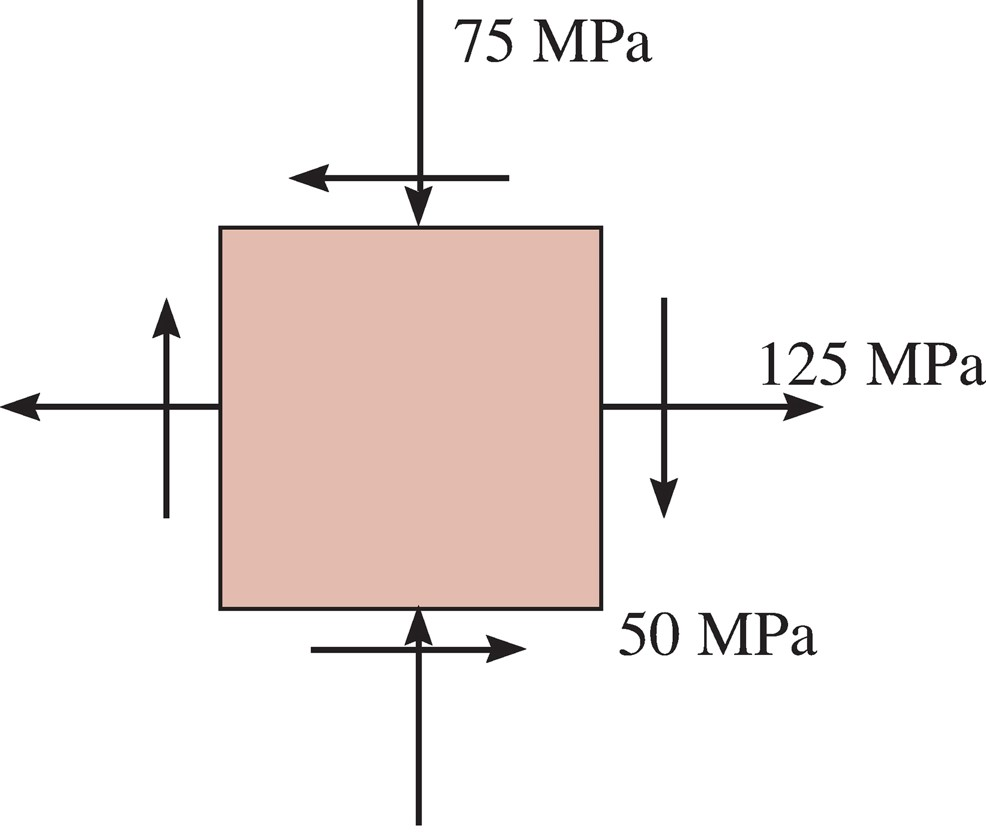
\includegraphics[width=0.6\linewidth]{9-17}
		\end{figure}

	\item For the stress state in Problem 1, find the principal stresses and maximum (in-plane) shear stress
		\newpage

	\item %9-20
		The stress state along two planes is known as shown.
		Find the normal stresses on plane $b-b$ and the principal stresses.
		\begin{figure}[H]
			\centering
			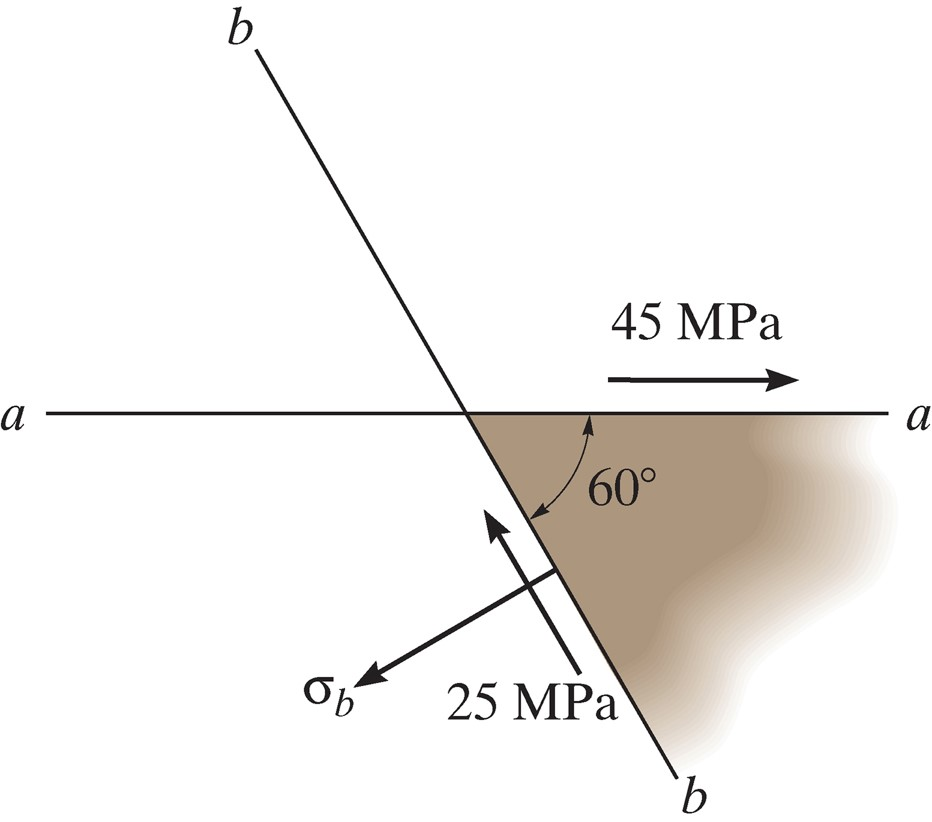
\includegraphics[width=0.6\linewidth]{9-20}
		\end{figure}

	\item %9-24
		The wood beam is subjected to a load of $ 	\SI{12 }{kN}  $.
		If grains of wood in the beam at point $A$ make an angle of $25^\circ$ with the horizontal as shown find the normal and shear stress that act perpendicular to the grains.
		\begin{figure}[H]
			\centering
			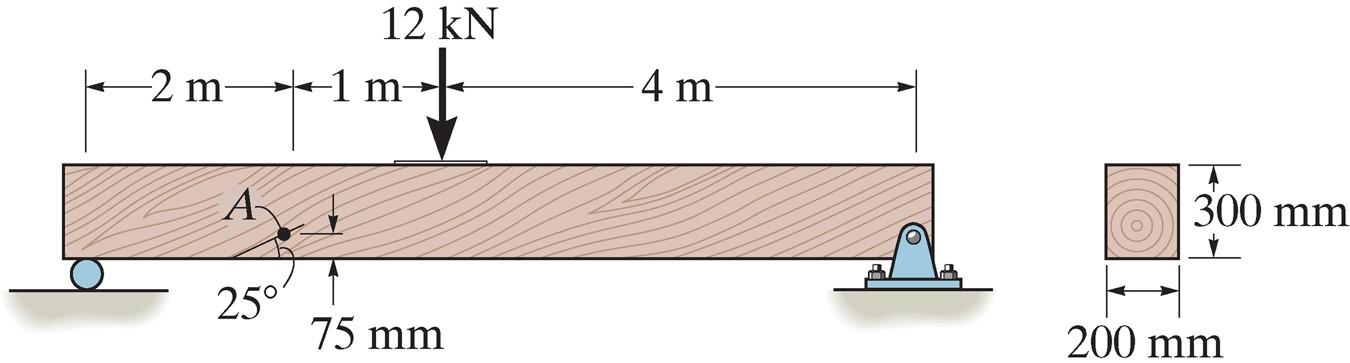
\includegraphics[width=0.8\linewidth]{9-24}
		\end{figure}
		\newpage

	\item Draw Mohr's circle for the stress state in problem 4 and use it to estimate the principal stresses.

	\item %10-25
		The $45^\circ$ strain rosette is mounted on the surface of a shell with the following readings: $\epsilon_a = -200 \mu \epsilon$, $\epsilon_b = 300 \mu \epsilon$ and $\epsilon_c = 250 \mu \epsilon$.
		Find the in-plane principal strains.
		\begin{figure}[H]
			\centering
			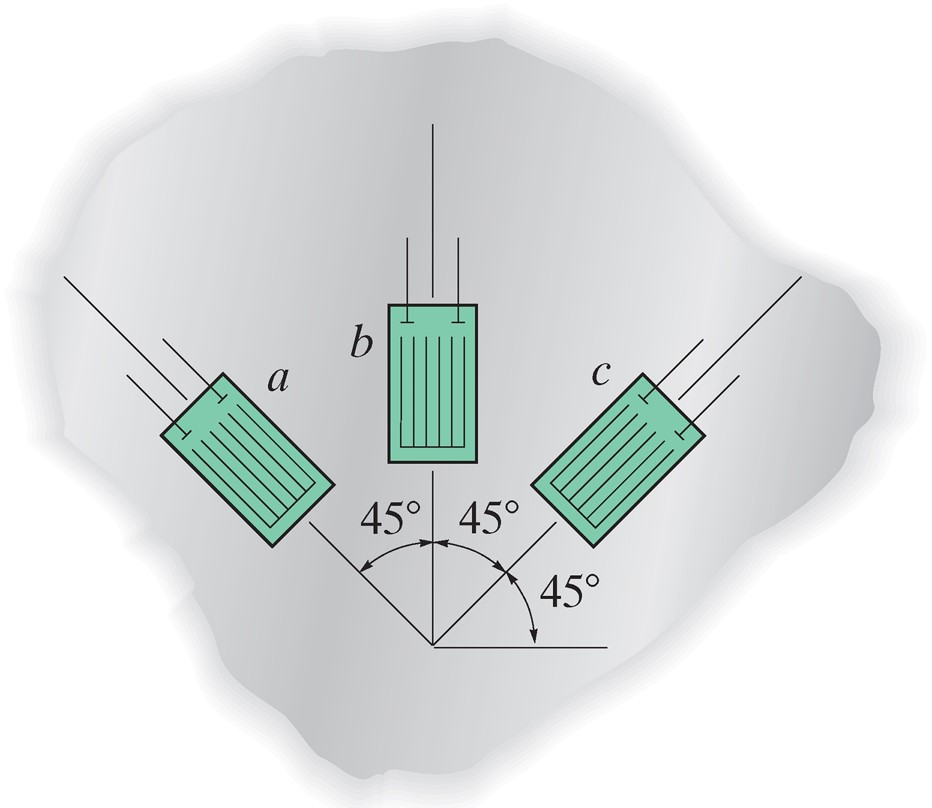
\includegraphics[width=0.6\linewidth]{10-25}
		\end{figure}
		\newpage

	\item %10-45
		A material is subjected to principal stresses $\sigma_x$ and $\sigma_y$.
		Find the orientation, $\theta$, of the strain gage so that its reading of normal strain corresponds only to $\sigma_y$, not $\sigma_x$.
		The relevant material constants for this problem are $E$ and $\nu$ (express answer in terms of these)
		\begin{figure}[H]
			\centering
			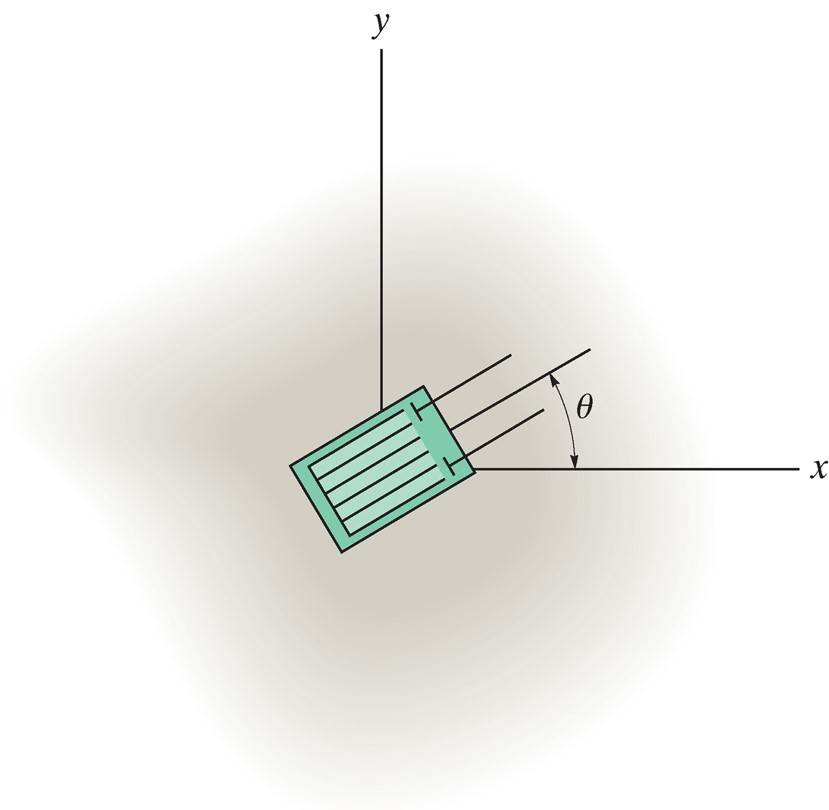
\includegraphics[width=0.6\linewidth]{10-45}
		\end{figure}

\end{enumerate}
\end{document}
